\lfoot{Autor: Raphael Simsek}
\subsubsection{OBD II}
\label{subsec:obd2}

\paragraph{Definition}
Häufig ist die OBD-II Schnittstelle bei Autofahrern für das Auslösen von Problemen bekannt. Genannte Probleme stammen vielfach von \textit{Error-Codes oder Diagnostic Trouble Codes (DTCs)}, welche aus der \textit{Engine Control Unit}  ausgeworfen werden und häufig das komplette Vehikel unfreiwillig stilllegen. Derartige DTCs müssen folglich in einer Fachwerkstatt reseted werden. Weitere Informationen zum Hintergrund des System sind unter Auslesen in diesem Kapitel auffindbar. 
Die OBD-II Schnittstelle ist eine standardisierte Schnittstelle. Die Schnittstelle verschafft Zugriff auf Daten des Motormanagements. Für die Auslesung der Daten des Motormanagments ( \textit{Engine Control Unit}) ist ein passendes Auslesegerät nötig. Sie hat unterschiedliche Versionen, welche auf die verschiedenen Kontinente aufgeschlüsselt wurden. Die Schnittstelle wird vor allem für das Auslesen vom Fehlercodes aus dem Motormanagement verwendet. Sie kann aber zusätzlich dazu auch durch standardisierte Datenabfragen (Mode 01) Echtzeit Daten liefern.

\paragraph{Standardisierung}
Die Geschichte der Standardisierung sieht folgender maßen aus\cite{SIMR.CH2-obd2.Timeline}:
\begin{itemize}
	\item 1980: General Motors führt \textit{assembly line diagnostic link (ALDL)} ein
	\item 1988: Die \textit{Society of Automotive Engineers (SAE)} rät einen standardisierten Konnektor mit Testsignalen an
	\item 1991: \textit{California Air Resources Board (CARB)} fordert, dass alle Autos die ab 1991 in Kalifornien verkauft werden, Basisfunktionalität mit OBD aufweisen
	\item 1996: Die OBD-II Spezifikation wird für alle Autos die in den USA verkauft werden Pflicht
	\item 2001: EOBD wird obligatorisch für Benzin-Fahrzeuge innerhalb der EU
	\item 2003: EOBD wird obligatorisch für Diesel-Fahrzeuge innerhalb der EU
\end{itemize}
Die OBD-II Schnittstelle wurde zuerst in den USA etabliert, wo sie auch 1996 zuerst verpflichtend wurde. Zusätzlich wurde EOBD als Standard definiert, womit die europäische Umsetzung des OBD-II Standards beschrieben wird \cite{SIMR.CH2-obd2.EUP-D98/69/EC}. Der wesentliche Unterschied ist die Standardisierung. Die ist zwar technisch zwischen SAE J1962 und ISO/DIS 15031 equivalent, es wurden aber trotzdem unterschiedliche Namen gewählt \cite{SIMR.CH2-obd2.SAEJ1962}. Ferner gibt es einen australischen \cite{SIMR.CH2-obd2.AU-MVSA1989} und eine japanischen Standard.

\paragraph{Charakterisierung}
Außerdem wurde innerhalb der Standardisierung die Form des Konnektors festgelegt. Dieser ist entweder als OBD-II A oder B Konnektor definiert. Der A Konnektor ist für alle Fahrzeuge mit 12 V Bordspannung und hat, siehe Abbildung \ref{Fig:imgOBDA}, die Form eines D mit einer Nut in der Mitte, um die Pins zu behausen. Der B Konnektor, siehe Abbildung \ref{Fig:imgOBDB},  allerdings ist dieser Konnektor für Fahrzeuge mit 24V Bordspannung. Diese sind beispielsweise Lastkraftfahrzeuge. Bei OBD II Typ B ist die Nut in der Mitte unterbrochen, um es unmöglich zu machen einen männlichen Konnektor des A-Typs einzustecken. Dieser Konnektor könnte nämlich aufgrund von Überspannung zu einem Defekt führen. Es ist also der B Konnektor sowohl mit A und B kompatibel, allerdings ist der A Konnektor nur mit seinesgleichen verwendbar.

\begin{figure}[!htb]\centering
   \begin{minipage}{0.49\textwidth}
     \frame{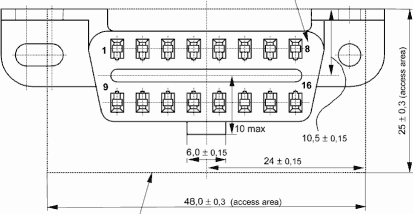
\includegraphics[width=\linewidth]{images/j1962f_type_a}}
     \caption{Typ A, OBD II Konnektor \cite{SIMR.CH2-obd2.OBDIITypeA}}\label{Fig:imgOBDA}
   \end{minipage}
   \begin {minipage}{0.49\textwidth}
     \frame{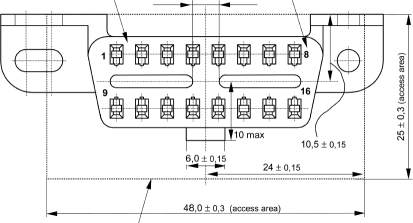
\includegraphics[width=\linewidth]{images/j1962f_type_b}}
     \caption{Typ B, OBD II Konnektor \cite{SIMR.CH2-obd2.OBDIITypeB}}\label{Fig:imgOBDB}
   \end{minipage}
\end{figure}


\paragraph{Positionierung / Lokalisierung\nextline}
Die OBD II Schnittstelle muss innerhalb der EU bei allen PKW mit Benzinmotor ab 2001 und bei allen PKW mit Dieselmotor ab 2004 vom Fahrer erreichbar verbaut sein. Aus diesem Grund wird die OBD-II Schnittstelle von gängigen Automobilherstellern oft fahrerseitig im Bereich der Pedale. Die Schnittstelle wird häufig in  Bereich der Fahrzeugsicherungen angebracht (siehe Abb. \ref{Fig:imgOBDSicherungskasten}):
\begin{figure}[!htb]\centering
	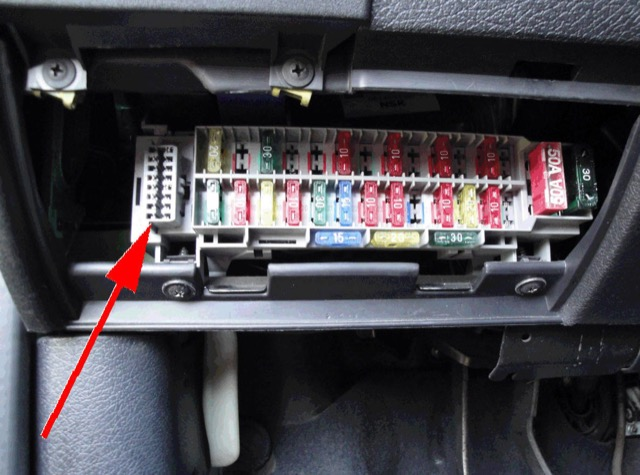
\includegraphics[width=0.5\textwidth]{images/obdSicherungskasten}
	\caption{OBD-II Konnektor im Sicherungskasten bei einem Opel Corsa B 1.0 12 V \cite{SIMR.CH3-obd2.OBDSicherungskasten}}\label{Fig:imgOBDSicherungskasten}
\end{figure}
Exemplarisch können Sie hier die Lokalisierung der OBD II Schnittstelle an einem Golf VI erkennen. Diese Schnittstelle ist hier unterhalb einer ohne Werkzeug entfernbaren Abdeckung versteckt. Wie auf dem Foto erkennbar ist die Schnittstelle hier im Fußraum der Fahrerseite, links der Pedale platziert.

\begin{figure}[!htb]\centering
	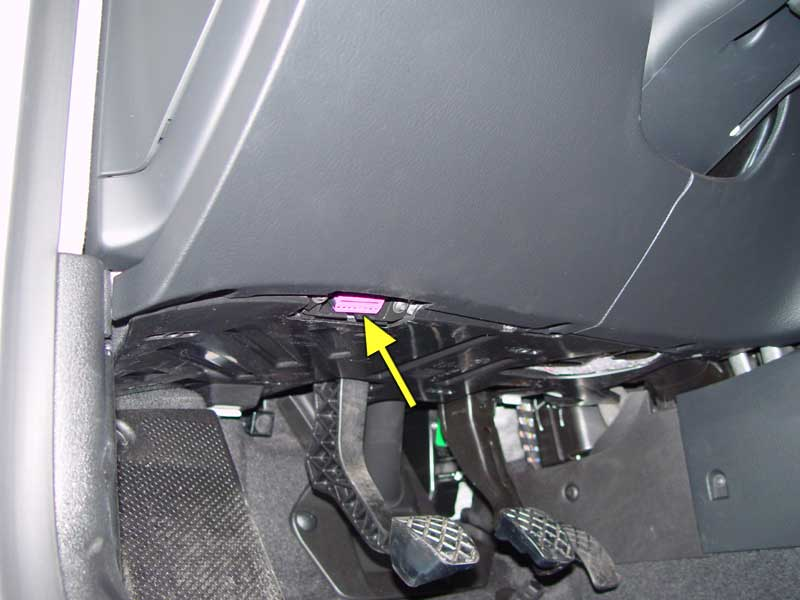
\includegraphics[width=0.5\textwidth]{images/golfobd}
	\caption{OBD II Konnektor bei einem Golf VI \cite{SIMR.CH2-obd2.GolfOBD}}\label{Fig:Data3}
\end{figure}

Bei einem BMW 3er E90 ist der OBD Konnektor hinter der linken Fußraumverkleidung der Fahrerseite zu finden. Er wurde unter einer kleinen Abdeckung, welche mit \"OBD\" beschriftet ist, verdeckt. Die OBD Schnittstelle ist hier vertikal angeordnet.

\begin{figure}[!htb]\centering
	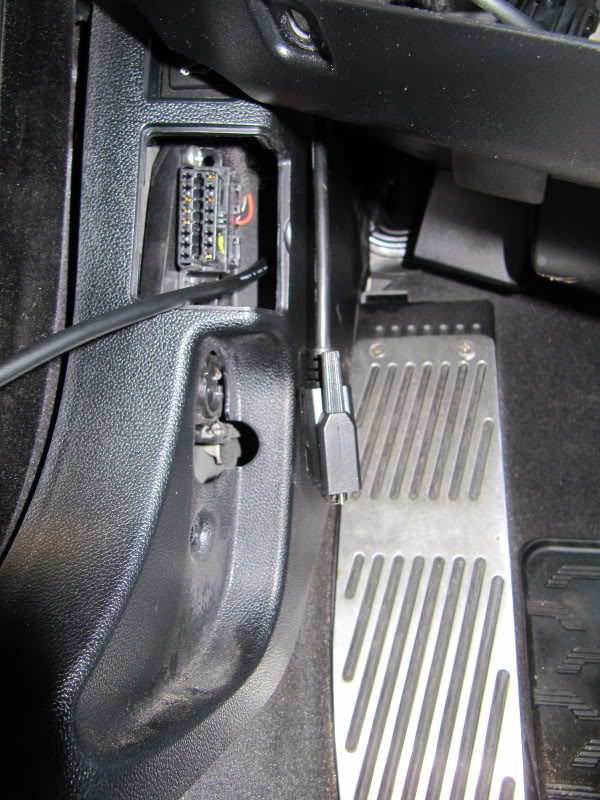
\includegraphics[width=0.6\textwidth]{images/3erobd}
	\caption{OBD II Konnektor bei einem BMW 3er E90 \cite{SIMR.CH2-obd2.3erOBD}}\label{Fig:Data3}
\end{figure}

\paragraph{Auslesen}
Das bei der OBD-II Schnittstelle verwendete Datenübertragungsprotokoll basiert auf einem \textit{Controller Area Network (CAN)}-Bus. Dies das Auslesen mit diesem Bus erfolgt in der Regel so:
\begin{itemize}
	\item Der Mechaniker schließt ein Auslesegerät an die OBD-II Schnittstelle des Fahrzeugs an
	\item Der Mechaniker gibt die gewollte PID ein
	\item Das Auslesegerät schickt die Anfrage an den Bus des Fahrzeugs (Protokolle: CAN, VPW, PWM, ISO, KWP vor 2008; nach 2008 ausschließlich CAN)
	\item Ein Gerät innerhalb des Bus erkennt dann dass es für den PID zuständig ist, der abgefragt wurde und liefert den Wert der PID an den Bus
	\item Das Auslesegerät ließt die Antwort aus und zeigt sie dem Mechaniker, welcher dann entscheidet welche weiteren Schritte nötig sind
\end{itemize}

Das Datenprotokoll des CAN Bus ist das \textit{Standard Frame CAN 2.0A}. Dieses ist, wie in \ref{table:CANProtokoll} erkennbar, so definiert:
\begin{table}[!htb]
\centering
\caption{CAN Protokoll Aufbau}
\label{table:CANProtokoll}
\begin{tabular}{|l|l|l|l|l|l|l|l|l|l|}
\hline
\begin{tabular}[c]{@{}l@{}}Start\\ 1 Bit\end{tabular} & \begin{tabular}[c]{@{}l@{}}Identifier\\ 11 Bit\end{tabular} & \begin{tabular}[c]{@{}l@{}}RTR\\ 1 Bit\end{tabular} & \begin{tabular}[c]{@{}l@{}}IDE\\ 1 Bit\end{tabular} & \begin{tabular}[c]{@{}l@{}}r0\\ 1 Bit\end{tabular} & \begin{tabular}[c]{@{}l@{}}DLC\\ 4 Bit\end{tabular} & \begin{tabular}[c]{@{}l@{}}DATA\\ 0...8 Byte\end{tabular} & \begin{tabular}[c]{@{}l@{}}CRC\\ 15 Bit\end{tabular} & \begin{tabular}[c]{@{}l@{}}ACK\\ 2 Bit\end{tabular} & \begin{tabular}[c]{@{}l@{}}EOF+IFS\\ 10 Bit\end{tabular} \\ \hline
\end{tabular}
\end{table}
Genauer beschrieben bedeuten die Standards folgendes:
\begin{itemize}
	\item Start: Synchronisationsbit
	\item Identifier: Informationen für den Empfänger
	\item RTR: Daten- (dominant) und Datenanforderungstelegramm (rezessiv)
	\item IDE: Identifier Extention
	\item r0: reserviert
	\item DLC: Längeninformation der nachfolgenden Daten
	\item DATA: Daten des Telegramms
	\item CRC: Fehlercode für die vorangegangen Informationen, Fehlererkennung
	\item ACK: Rückmeldung von anderen Teilnehmern des Bus
	\item EOF: Ende des Telegramms (7 rezessive Bits)
	\item IFS: Timeout der korrekten Übertragung des Telegramms \cite{SIMR.CH3-obd2.CANBus}
\end{itemize}
Schlussfolgernd ist der CAN Bus also ein sehr einfaches Bus Protokoll, weshalb die Elektronik innerhalb eines Autos sehr einfache Netzwerkarchitekturen verwenden können.

Die OBD-II Schnittstelle muss laut Norm zur Verfügung stellen, welche Daten die Schnittstelle ausgeben kann und welche Standards (siehe am Beginn des Kapitels) die Schnittstelle unterstützt \cite{SIMR.CH2-obd2.PIDMustHave}. Diese werden über standardisierte Kennnummern, sogenannte PID (Parameter IDentification). Da Fahrzeughersteller fast immer noch zusätzliche Daten bereitstellen, können alle unterstützten PIDs ausgelesen werden. Vorgehensweise mittels des verwendeten Bluetooth ELM 327 Dongles: 

\begin{enumerate}
	\item Verbindung aufbauen
	\begin{enumerate}
		\item Verbindung mit Bluetooth OBD-II ELM327 Chip aufbauen
		\item Verbindung zum seriellen COM-Port aufbauen 
	\end{enumerate}
	\item Mode \# + PID \# (zusammen also 0100/0120/0140/0160/0180/...) abfragen
	\item Zurückgegebene 4 Byte von Hexadezimal zu Binär umrechnen
	\item In eine Tabelle einfügen und überprüfen welche PID's unterstützt sind
\end{enumerate}

Jedes Bit entspricht einer unterstützten PID. In Tabelle 1 wird ein typisches Ergebnis einer PID-Abfrage „BE1FA813“ gezeigt.

\begin{table}[!htb]
\centering
\resizebox{\columnwidth}{!}{%
\begin{tabular}{|l|c|c|c|c|c|c|c|c|c|c|c|c|c|c|c|c|}
\hline
Hexadecimal & \multicolumn{4}{c|}{B} & \multicolumn{4}{c|}{E} & \multicolumn{4}{c|}{1} & \multicolumn{4}{c|}{F} \\ \hline
Binary & 1 & 0 & 1 & 1 & 1 & 1 & 1 & 0 & 0 & 0 & 0 & 1 & 1 & 1 & 1 & 1 \\ \hline
Supported? & \cellcolor[HTML]{9AFF99}Yes & \cellcolor[HTML]{FD6864}No & \cellcolor[HTML]{9AFF99}Yes & \cellcolor[HTML]{9AFF99}Yes & \cellcolor[HTML]{9AFF99}Yes & \cellcolor[HTML]{9AFF99}Yes & \cellcolor[HTML]{9AFF99}Yes & \cellcolor[HTML]{FD6864}No & \cellcolor[HTML]{FD6864}No & \cellcolor[HTML]{FD6864}No & \cellcolor[HTML]{FD6864}No & \cellcolor[HTML]{9AFF99}Yes & \cellcolor[HTML]{9AFF99}Yes & \cellcolor[HTML]{9AFF99}Yes & \cellcolor[HTML]{9AFF99}Yes & \cellcolor[HTML]{9AFF99}Yes \\ \hline
PID number & 1 & 2 & 3 & 4 & 5 & 6 & 7 & 8 & 9 & 0A & 0B & 0C & 0D & 0E & 0F & 10 \\ \hline
Hexadecimal & \multicolumn{4}{c|}{A} & \multicolumn{4}{c|}{8} & \multicolumn{4}{c|}{1} & \multicolumn{4}{c|}{3} \\ \hline
Binary & 1 & 0 & 1 & 0 & 1 & 0 & 0 & 0 & 0 & 0 & 0 & 1 & 0 & 0 & 1 & 1 \\ \hline
Supported? & \cellcolor[HTML]{9AFF99}Yes & \cellcolor[HTML]{FD6864}No & \cellcolor[HTML]{9AFF99}Yes & \cellcolor[HTML]{FD6864}No & \cellcolor[HTML]{9AFF99}Yes & \cellcolor[HTML]{FD6864}No & \cellcolor[HTML]{FD6864}No & \cellcolor[HTML]{FD6864}No & \cellcolor[HTML]{FD6864}No & \cellcolor[HTML]{FD6864}No & \cellcolor[HTML]{FD6864}No & \cellcolor[HTML]{9AFF99}Yes & \cellcolor[HTML]{FD6864}No & \cellcolor[HTML]{FD6864}No & \cellcolor[HTML]{9AFF99}Yes & \cellcolor[HTML]{9AFF99}Yes \\ \hline
PID number & 11 & 12 & 13 & 14 & 15 & 16 & 17 & 18 & 19 & 1A & 1B & 1C & 1D & 1E & 1F & 20 \\ \hline
\end{tabular}
}
\caption{Tabelle zur bitweisen Verarbeitung der Hexadezimal Zeichenkette \cite{SIMR.CH2-obd2.HextoBinary}}
\label{tableHextoPID}
\end{table}

Es wurden innerhalb des Projektes ausschließlich Daten des PID Mode 01 (Realtime Data) verwendet. Grundsätzlich sind alle Mode 01 PIDs zwischen 00 und 87 bezüglich ihrer Einheiten und Bereiche standardisiert. Die PIDs zwischen A0 und E0 sind komplett frei für Autohersteller verfügbar um abseits der Norm eigene Daten einzupflegen. 

Während des Projektes wurden die PIDs 04 - Calculated engine load [\%] und 0C - Rotations per Minute [0-16.383,75] für den Schaltvorschlag verwendet, wozu im nächsten Abschnitt genauere Informationen gefunden werden können. Für die Errechnung des \ce{CO2}-Ausstoßes wurde PID 43 - absolute load value [0-25.700] und 5E - engine fuel rate [L/h] eingesetzt.
PID 04 wurde verwendet um auf der vertikalen Achse, der Abbildung xy, eingetragen zu werden. PID 0C wurde für die horizontale selbiger Abbildung verwendet.

\clearpage % DO NOT REMOVE